%%%%%%%%%%%%%%%%%%%%%%%%%%%%%%%%%%%%% 
%% LE2I beamer template
%% Guillaume Lemaitre, October 2014
%%%%%%%%%%%%%%%%%%%%%%%%%%%%%%%%%%%%% 

\documentclass{beamer}

\usepackage[utf8]{inputenc}
\usepackage[T1]{fontenc} 
\usetheme{le2i} 

%% The amssymb package provides various useful mathematical symbols
\usepackage{amssymb}
%% The amsthm package provides extended theorem environments
\usepackage{amsthm}

%% amsmath for math environment
\usepackage{amsmath}

\DeclareMathOperator*{\argmin}{arg\,min}
\DeclareMathOperator*{\argmax}{arg\,max}
\DeclareMathOperator*{\sign}{sign}

%% figure package
\usepackage{epsf,graphicx}
\usepackage{epstopdf}
\usepackage{subfigure}
\usepackage{transparent}

%% In order to draw some graphs
\usepackage{tikz,xifthen}
\usepackage{tikz-qtree}
\usepackage{adjustbox}
\usetikzlibrary{decorations.pathmorphing}
\usetikzlibrary{fit}
\usetikzlibrary{backgrounds}
\usetikzlibrary{shapes,arrows,shadows}
\usetikzlibrary{calc,decorations.pathreplacing,decorations.markings,positioning}
\usetikzlibrary{snakes,decorations.text,shapes,patterns}
% \usepackage{scalefnt,lmodern,booktabs}

%% Package for cross and tick symbols
\usepackage{pifont}
\newcommand{\tick}{\color{green!60!black!80}\ding{51}}
\newcommand{\cross}{\color{red!60!black!80}\ding{55}}

\title{Image Enhancement}
\author{Guillaume Lemaitre}
%\date{Define the event \\ day\textsuperscript{th} Month Year}

\institute{Universit\'e de Bourgogne} 

%% Uncomment if you want to avoid thousand of bullet inside the menu
% \usepackage{etoolbox}
% \makeatletter
% \patchcmd{\slideentry}{\advance\beamer@xpos by1\relax}{}{}{}
% \def\beamer@subsectionentry#1#2#3#4#5{\advance\beamer@xpos by1\relax}%
% \makeatother

\begin{document}

% Show the title page
\begin{frame}
  \titlepage
\end{frame}

% Show the table of contents
\begin{frame}
  \tableofcontents[sectionstyle=show,subsectionstyle=show,subsubsectionstyle=hide]
\end{frame}

%---------------------
\section{Spatial Filtering}
\begin{frame}
\frametitle{Spatial Filtering}
\begin{itemize}
	\item Use of spatial masks for image processing 
	\item Linar and Nonlinear 
\end{itemize}
\begin{block}{Different types}
	\begin{itemize}
	\item Low-pass filters 
	\item High-pass filters 
	\item Band-pass filters
	\end{itemize}
\end{block}
\end{frame}

%------------
\begin{frame}
\frametitle{Spatial Filtering}
\begin{itemize}
	\item \textbf{Low-pass} filters eliminate or attenuate high frequency component ({\color{blue} sharp image details}) in the frequency domain, and result in image {\color{blue} blurring}.
	\item \textbf{High-pass} filters eliminate and attenuate the low frequency components and result in {\color{blue} sharpening edges} and other sharp details. 
	\item \textbf{Band-pass} filter, remove selected frequency regions between low and high frequencies. 
\end{itemize}
\end{frame}
%----------
\begin{frame}
\frametitle{Spatial Filtering}
\framesubtitle{Linear filtering}
Linear filtering of an image $f$ of size $M \times N$ with a filter mask of size $m \times n$: 
$$g(x,y) = \sum^{a}_{s=-a}\sum^{b}_{t=-b} w(s,t)f(x+s, y+t)$$
\noindent $a = (m-1)/2$ and $b = (n-1)/2$\\
for $x = 0, 1, ..., M-1$ and $y = 0,1,..., N-1$\\
{\color{blue}Also called convolution (primarily in the frequency domain)}
\end{frame}
%----------
\begin{frame}
\frametitle{Spatial filter}
\framesubtitle{Linear filtering}
The basic approach is to sum products between the mask coefficients and the intensities of the pixels under the mask at a specific location in the image. \\
for $3 \times 3$ filter: 
$$R = w_{1}z_{1}+w_{2}z_{2}+...+w_{9}z_{9}$$
\end{frame}
%----------
\begin{frame}
\frametitle{Spatial Filtering}
\framesubtitle{Linear filtering}
\begin{center}
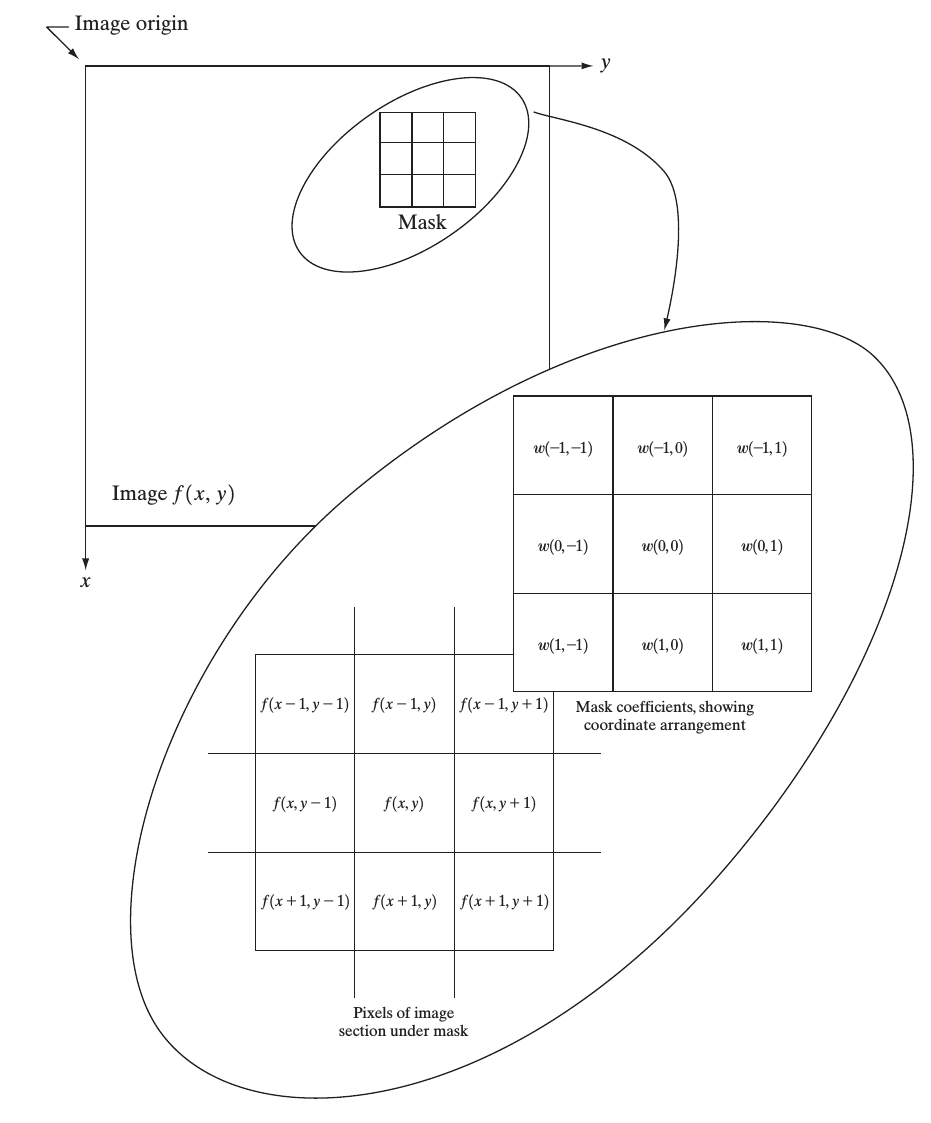
\includegraphics[scale=0.23]{images/Spatial2.png}
\end{center}
\end{frame}
%-----------
\begin{frame}
\frametitle{Spatial Filtering}
\framesubtitle{Smoothing linear filter}
\begin{itemize}
\item  Replacing the value of every pixel in an image by the average of the gray levels in the neighborhood defined by the filter mask.
\item Averaging filter 
\item {\color{red} Blurring the edges}
\item Two $3\times 3$ smoothing (averaging) filter masks. The constant multiplier in front of each mask is equal to the sum of the values of its coefficients, as is required to compute an average.
\begin{center}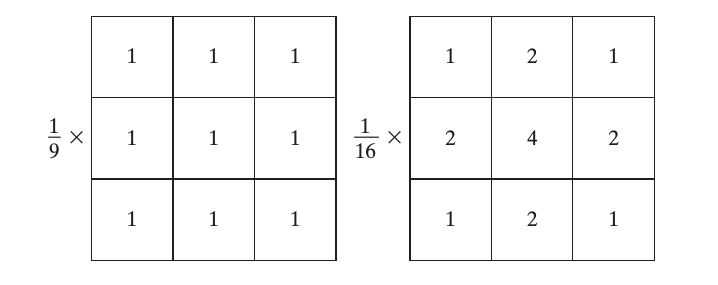
\includegraphics[scale=0.4]{images/Spatial3.png}\end{center}
\end{itemize}
\end{frame}
%-----------
\begin{frame}
\frametitle{Spatial Filtering}
\framesubtitle{Smoothing linear filter}
Results of smoothing with square averaging filter masks of sizes n=3, 5, 9, 15, and 35, respectively. 
\begin{center}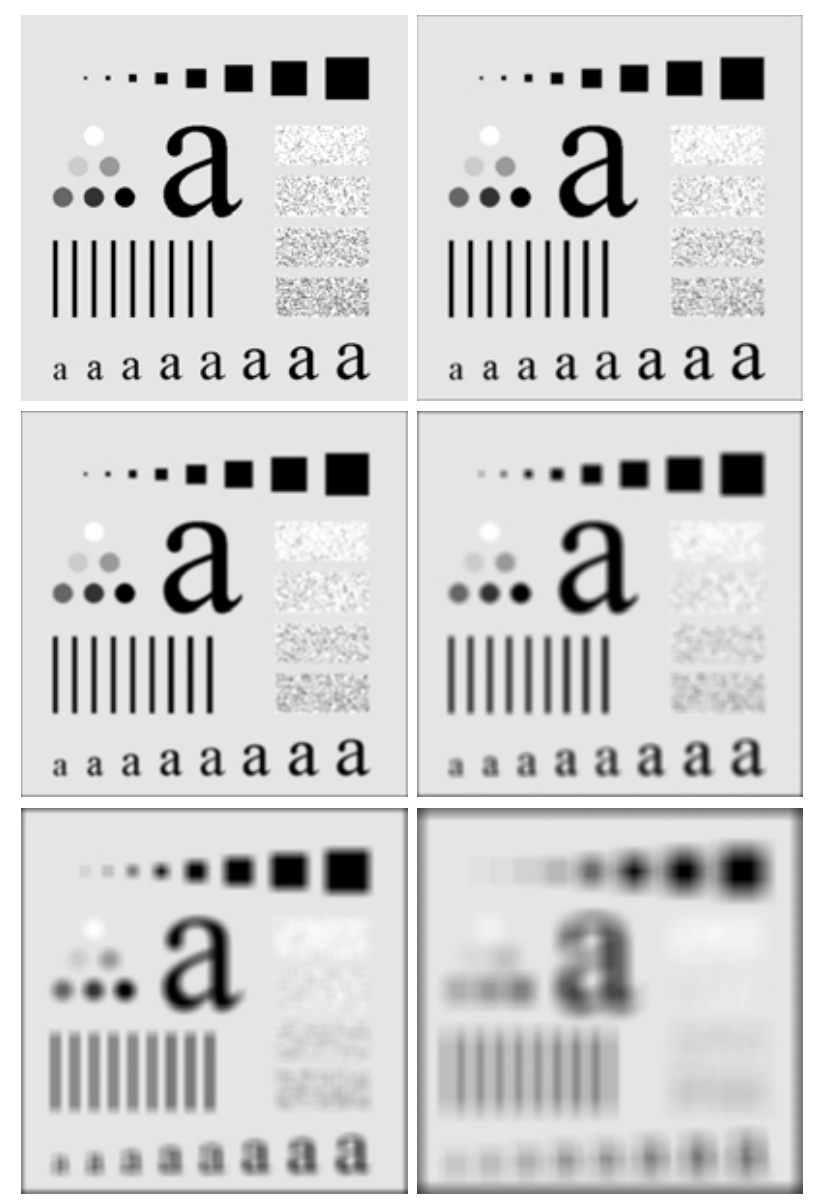
\includegraphics[scale=0.19]{images/Spatial4-averagefilter.png}\end{center}
\end{frame}

%----------
\begin{frame}
\frametitle{Spatial Filtering}
\framesubtitle{Smoothing linear filter}
(b) Image processed by $15 \times 15$ average mask. (c) Result of thresholding 
\begin{center}
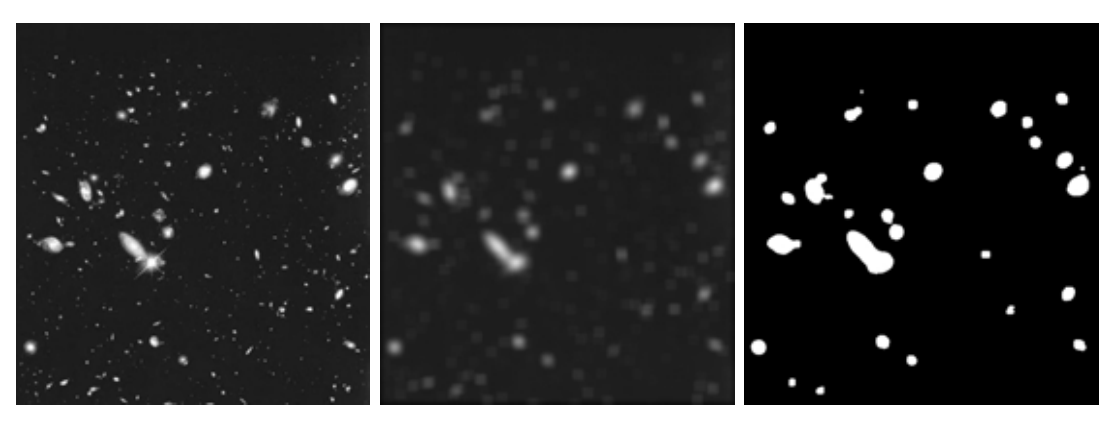
\includegraphics[scale=0.3]{images/Spatial5-averagefilter.png}
\end{center}
\end{frame}
%-----------
\begin{frame}
\frametitle{Spatial Filtering}
\framesubtitle{Smoothing nonlinear filter}
Median filtering also used for noise elimination. 
\begin{itemize}
\item The gray level of each pixel is replaced by the median gray levels in the neighborhood of the pixel instead of the average.
\item X-ray image of the circuit board corrupted by salt-and-pepper noise. Noise reduction with $3 \times 3$ average and median filter, respectively.
\item[]\begin{center}
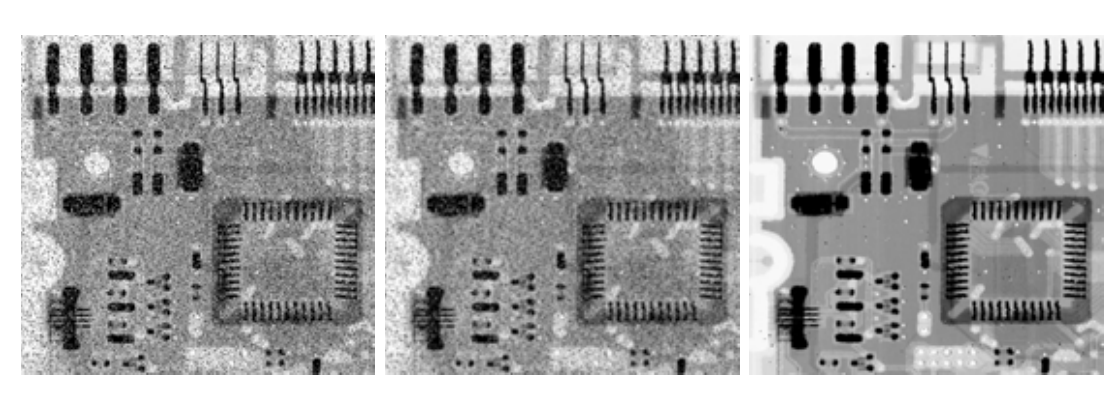
\includegraphics[scale=0.3]{images/Spatial6-averagemedian.png}
\end{center}  
\end{itemize}
\end{frame}
%---------
\begin{frame}
\frametitle{Spatial Filtering}
\framesubtitle{Sharpening filter}
\begin{itemize}
\item To highlight fine detail or to enhance blurred detail. 
\begin{itemize}
\item smoothing ~ integration
\item sharpening ~ differentiation
\end{itemize}
\end{itemize}
\begin{block}{ Categories of sharpening filters: }
\begin{itemize}
\item Derivative operator 
\item Basic high-pass spatial filter 
\item High-boost filtering 
\end{itemize}
\end{block}
\end{frame}
%------------
\begin{frame}
\frametitle{Spatial Filtering}
\framesubtitle{Sharpening filter - Derivative filter}
\begin{itemize}
\item First-order derivative 
$$\frac{\partial f}{\partial x} = f(x+1) - f(x)$$
\item Second-order derivative 
$$\frac{\partial^{2}f}{\partial x^{2}} = f(x+1)+f(x-1) - 2f(x)$$
\end{itemize}
\end{frame}
%-----------
\begin{frame}
\frametitle{Spatial Filtering}
\framesubtitle{Sharpening filter - Derivative filter}
\begin{center}
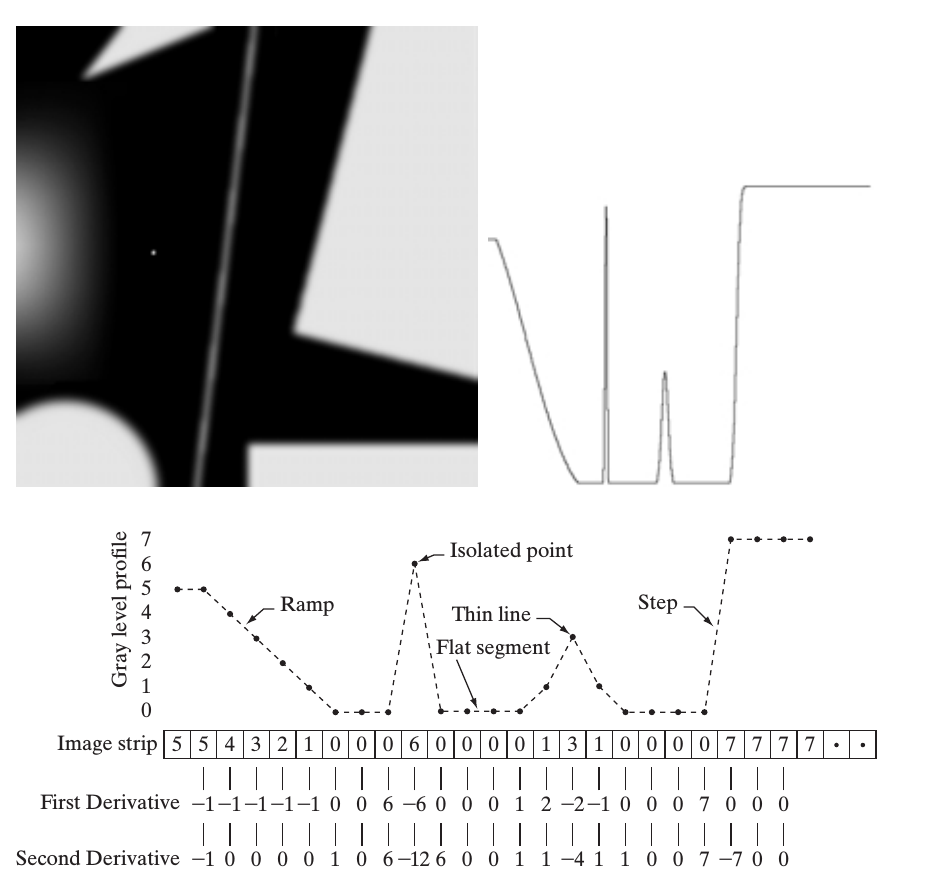
\includegraphics[scale=0.3]{images/Spatial7-derivative.png}
\end{center}		
\end{frame}
%-----------
\begin{frame}
\frametitle{Spatial Filtering}
\framesubtitle{Sharpening filter - Derivative filter}
\begin{itemize}
\item First derivative: 
	\begin{itemize}
	\item 0 in constant gray segments
	\item Non-zero at the onset of steps or ramps
	\item Non-zero along ramps
	\end{itemize}
\item Second derivative: 
	\begin{itemize}
	\item 0 in constant gray segments
	\item Non-zero at the onset and end of steps or ramps
	\item 0 along ramps of constant slope.
	\end{itemize}
\end{itemize}
\end{frame}
%-----------
\begin{frame}
\frametitle{Spatial Filtering}
\framesubtitle{Sharpening filter - Derivative filter}
\begin{itemize}
\item First-order derivatives generally produce thicker edges in an image
\item Second-order derivatives have a stronger response to fine detail, such as thin lines and isolated points
\item First-order derivatives generally have a stronger response to a gray-level step
\item Second-order derivatives produce a double response at step changes in gray level
\item Second-order derivatives have stronger response to a line than to a step and to a point than to a line
\end{itemize}
\end{frame}
%-----------
\begin{frame}
\frametitle{Spatial Filtering}
\framesubtitle{Sharpening filter - Basic Highpass Spatial filter}
\begin{itemize}
\item Cross section of frequency domain filter:
\begin{center}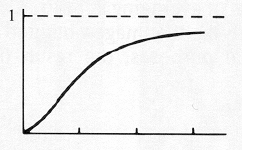
\includegraphics[scale=0.5]{images/HPS-f.png}\end{center} 
\item Cross section of spatial domain filter:
\begin{center}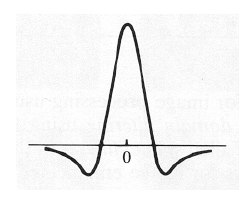
\includegraphics[scale=0.5]{images/HPS-S.png}\end{center} 
\end{itemize}
\end{frame}
%-----------
\begin{frame}
\frametitle{Spatial Filtering}
\framesubtitle{Sharpening filter - Basic Highpass Spatial filter}
\begin{itemize}
\item The filter should have positive coefficients near the center and negative in the outer periphery
\begin{center}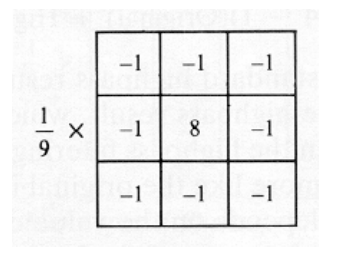
\includegraphics[scale=0.3]{images/HPF.png}\end{center}
\item The sum of the coefficients is 0, indicating that when the filter is passing over regions of almost stable gray levels, the output of the mask is 0 or very small.
\item Some scaling and/or clipping is involved to compensate for possible negative gray levels after filtering.
\end{itemize}
\end{frame}
%-----------
\begin{frame}
\frametitle{Spatial Filtering}
\framesubtitle{Sharpening filter - 2D, Second order derivatives}
\begin{itemize}
\item Isotropic filters, rotation invariant 
\item Laplacian (linear operator)
$$\triangledown^2 f = \frac{\partial^2 f}{\partial x^2}+ \frac{\partial^2 f}{\partial y^2}$$
\item Discrete version: 
$$\frac{\partial^2 f}{\partial x^2} = f(x+1,y) + f(x-1,y) -2f(x,y)$$
$$\frac{\partial^2 f}{\partial y^2} = f(x,y+1) + f(x,y-1) -2f(x,y)$$ 
\end{itemize}
\end{frame}
%-----------
\begin{frame}
\frametitle{Spatial Filtering}
\framesubtitle{Sharpening filter - 2D, Second order derivative}
\begin{itemize}
\item Digital implementation 
$$\triangledown^2 f = [f(x+1,y)+f(x-1,y)+f(x,y+1)+f(x,y-1)]-4f(x,y)$$
\item Two definitions, one is negative of the other
\[ g(x,y) =
  \begin{cases}
    f(x,y)-\triangledown^2 f(x,y)  & \quad \text{Center of the mask is negative} \\
    f(x,y)+\triangledown^2 f(x,y)  & \quad \text{Center of the mask is positive} \\
  \end{cases}
\]
\end{itemize}
\end{frame}
%----------
\begin{frame}
\frametitle{Spatial Filtering}
\framesubtitle{Sharpening filter - 2D, Second order derivative}
\begin{itemize}
\item Filtering and recovering the original part: 
\scriptsize{
$$ g(x,y) = f(x,y) - [f(x+1,y)+f(x-1,y)+f(x,y+1)+f(x,y-1)]+4f(x,y)$$
$$ g(x,y) = 5f(x,y) - [f(x+1,y)+f(x-1,y)+f(x,y+1)+f(x,y-1)]+4f(x,y)$$
}
\end{itemize}
\end{frame}
%----------
\begin{frame}
\frametitle{Spatial Filtering}
\framesubtitle{Sharpening filter - 2D, Second order derivative}
\begin{center}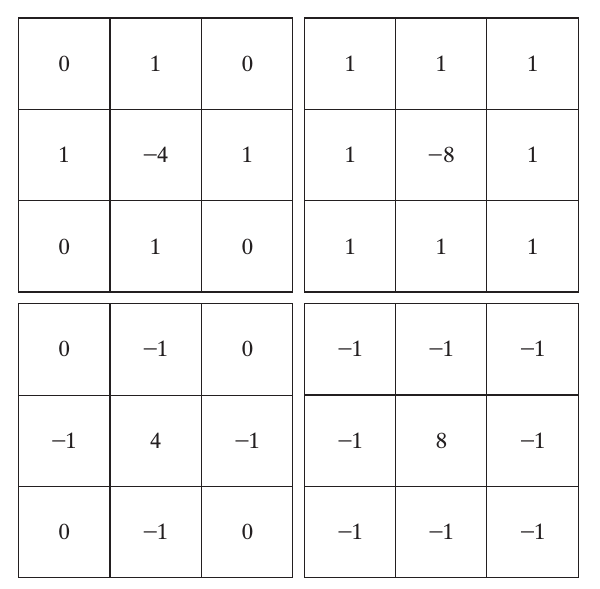
\includegraphics[scale=0.3]{images/Spatial7-laplacian.png}\end{center}
\end{frame}
%---------
\begin{frame}
\frametitle{Spatial Filtering}
\framesubtitle{Sharpening filter - 2D, Second order derivative}
Image of the north pole of the moon, laplacian filtered image, laplacian image scaled for display and image enhanced by laplacian, respectively.
\begin{center}
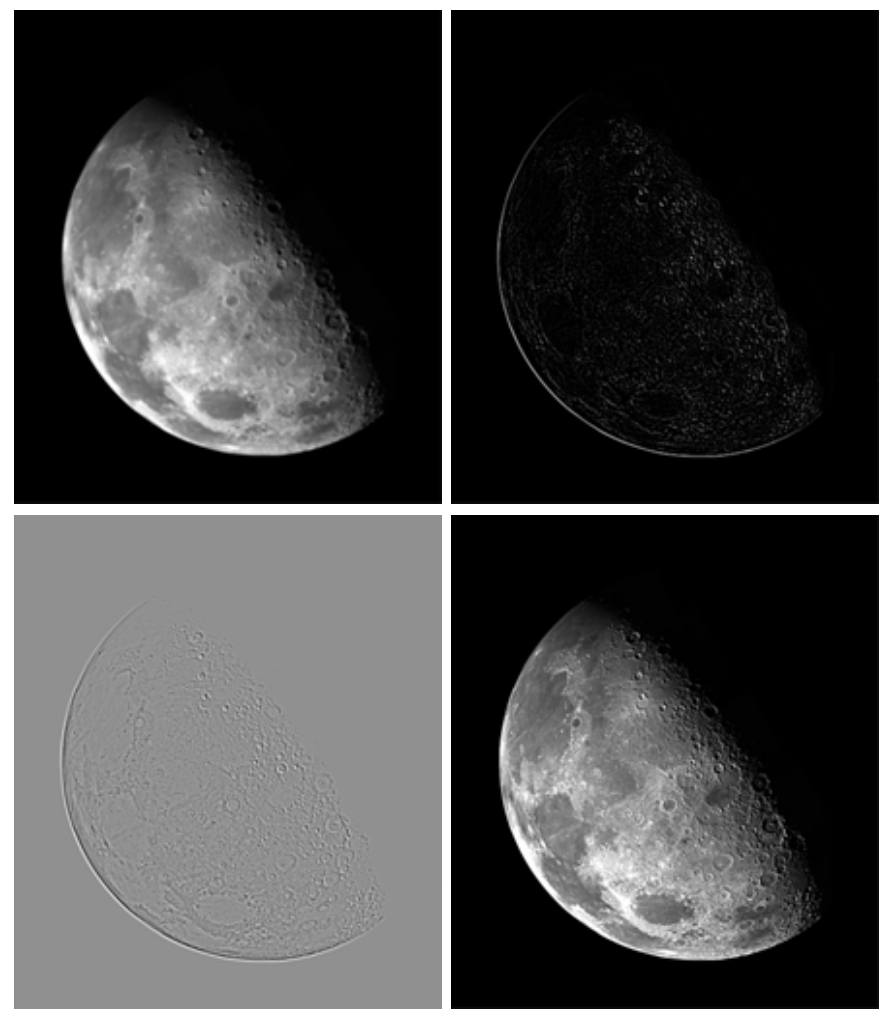
\includegraphics[width = 0.45\textwidth, height = 0.6\textheight]{images/Spatial8-laplacian-ex.png} 
\end{center}
\end{frame}
%-----------
\begin{frame}
\frametitle{Spatial Filtering}
\framesubtitle{Sharpening filter - High-boost filter}
\begin{itemize}
\item Unsharp masking : $f_{s}(x,y) = f(x,y)-\bar{f}(x,y)$
\item High-pass filtered image = original - low-pass filtered image. 
\item Consider $A$ as an amplification factor
$$ High-pass = A.original - low-pass(blurred)$$
$$ = (A-1).original + original - low-pass $$
$$ = (A-1).original + high-pass$$
\item A =1 --> Standard high-pass filter 
\item A >1 --> Enhanced image depending on the value of $A$   
\end{itemize}
\end{frame}
%-----------
\begin{frame}
\framesubtitle{Spatial Filtering}
\framesubtitle{Sharpening filter - High-boost filter}
\begin{center}
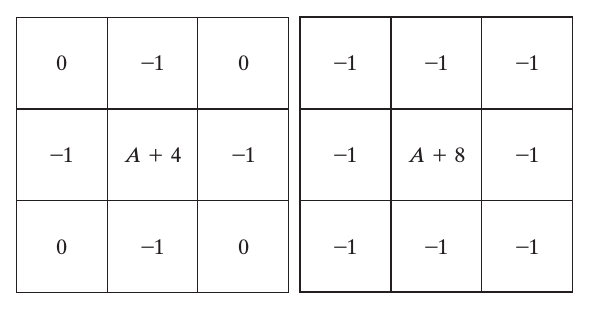
\includegraphics[scale=0.3]{images/Spatial9-HBF.png}
\end{center}
\end{frame}
%-----------
\begin{frame}
\frametitle{Spatial Filtering}
\framesubtitle{Gradient filter - first derivative}
\begin{itemize}
\item the most common method of differentiation in image processing
 $$\triangledown f = 
\begin{bmatrix}
G_x\\G_y
\end{bmatrix} = 
\begin{bmatrix}
\frac{\partial f}{\partial x}\\
 \frac{\partial f}{\partial y}
 \end{bmatrix}
$$
\item It is non-isotropic
\item Its magnitude (often call the gradient) is rotation invariant
$$\triangledown f = \vert G_{x} \vert + \vert G_{y} \vert = [(\frac{\partial f}{\partial x})^2 + (\frac{\partial f}{\partial x})^2]^{1/2} $$
\end{itemize}

\end{frame}
%-----------
\begin{frame}
\frametitle{Spatial Filtering}
\framesubtitle{Gradient filter - first derivative}
Different masks use to calculate the gradient of a region of interest with $z_{5}$ as a central pixel, Robert cross gradient masks middle row and  Sobel filters in the last row.
\begin{center}
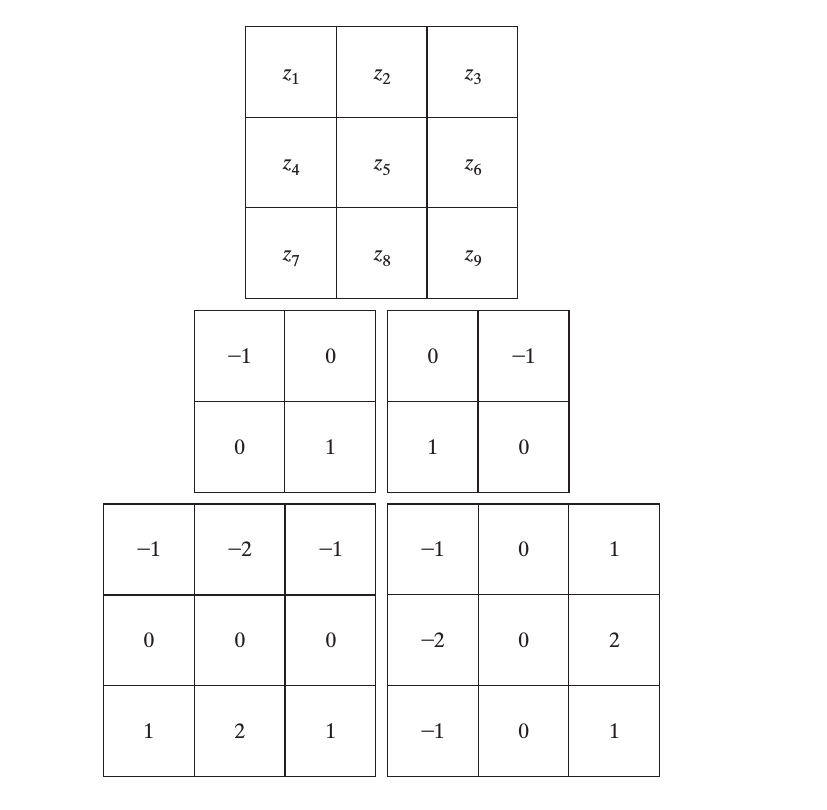
\includegraphics[scale=0.26]{images/Spatial10-gradient.png}
\end{center}
\end{frame}
%----------
\begin{frame}
\frametitle{Spatial Filtering}
\framesubtitle{Gradient filter - first derivative}
\begin{itemize}
\item Computation:
\item Cross differences as used in early development of digital image processing: 
$G_x = (z_9 - z_5)$, \quad $ G_y = (z_8 - z_6)$
\item Robert cross gradient: 
$$ \triangledown f \approx [(z_9 - z_5)^2 + (z_8 - z_6)^2]^{1/2}$$
\item Sobel filter 
\scriptsize{
$$ \triangledown f \approx \vert (z_7 + 2 z_8 + z_9) - (z_1 + 2 z_2 + z_3) \vert + \vert (z_3 + 2 z_9 + z_6) - (z_1 + 2 z_4 + z_7) \vert$$
}
\end{itemize}

\end{frame}

%----------
\begin{frame}
\frametitle{Spatial Filtering}
Whole body bone scane, laplacian image, sharpened image using the laplacian and sobel filtered image, respectively from right to left and first row to second. 
\begin{center}
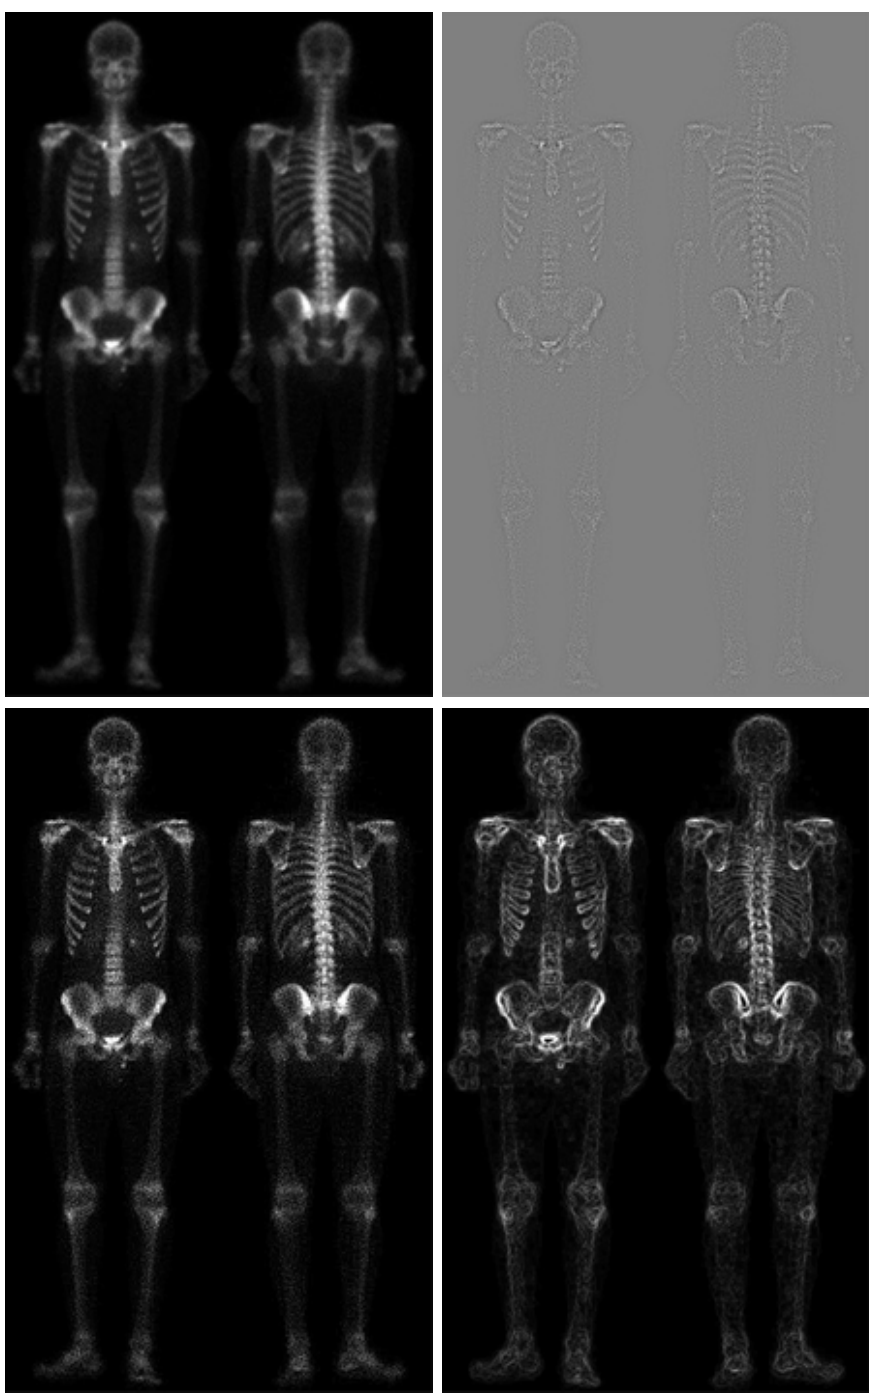
\includegraphics[scale=0.13]{images/Spatial12-ex1.png}
\end{center}
\end{frame}

%----------

\end{document}

%\begin{itemize}
%\item Also use neighborhood but do not use coefficients 
%\begin{itemize}
%\item median filter for noise reduction
%\end{itemize} 
%\end{itemize}
